
\subsection*{1.}

\begin{center}
\psset{xunit=2.75cm,yunit=2.75cm,showorigin=false,arrowsize=2pt 4}
\begin{pspicture}(-0.5,-0.75)(3,2)
\multido{\n=0.0+0.2}{16}{\psline[linewidth=0.75pt,linecolor=lightgray](\n,0)(\n,2)}
\multido{\n=0+0.2}{11}{\psline[linewidth=0.75pt,linecolor=lightgray](0,\n)(3,\n)}
\multido{\n=0+1}{4}{\psline[linewidth=0.75pt](\n,0)(\n,2)}
\multido{\n=0+1}{2}{\psline[linewidth=0.75pt](0,\n)(3,\n)}
\psaxes[linewidth=1.25pt]{->}(0,0)(0,0)(3.1,2)
\uput[dl](0,0){\textbf{O}}
\def\Func{2.71828 x neg exp x 4 mul mul}
\psplot[plotpoints=2000,linewidth=1.25pt,linecolor=blue]{0}{3}{\Func}
\uput[u](2.3,1){\blue $\mathcal{C}_f$}

\psline[linewidth=1.25pt,linecolor=green]{->}(1,1.471)(0,1.471) % Ligne horizontale
\psline[linewidth=1.25pt,linecolor=green]{->}(1,0)(1,1.471)    % Ligne verticale
\uput[l](0,1.471){\green $f(1) \approx 1,45$}

\psdots[dotstyle=*,dotscale=1.5,linecolor=red](1,1.471)
\uput[u](1.1,1.45){\red $A$}
\psline[linewidth=1pt,linecolor=red](0,0)(1,1.471)
\uput[u](0.71,1.575){\red $\mathcal{T}$}
\psline[linewidth=1pt,linecolor=red](0,0.607)(1.149,2)

\end{pspicture}
\end{center}

On lit un maximum approximatif \( f(1) \approx 1{,}45 \).

\subsection*{2.}

Pour tout réel \( x \) de \( \mathbb{R} \), donc en particulier de l'intervalle \( [0 \,;\, 3] \) :
\[
f'(x) = 4\e^{-x} - 4x\e^{-x} = \e^{-x} (4 - 4x) = 4\e^{-x} (1 - x).
\]

\subsection*{3.}

On sait que pour tout réel \( x \), \( \e^{-x} > 0 \), donc le signe de \( f'(x) \) est celui de \( 1 - x \).

Donc \( f'(x) > 0 \) si et seulement si \( 0 < x < 1 \) et \( f'(x) < 0 \) si et seulement si \( 1 < x < 3 \).

Tableau de signes : voir question 4.

\subsection*{4.}

D'après la question précédente, on en déduit que :
\begin{enumerate}[label=-]
    \item \( f \) est croissante sur \( [0 \,;\, 1] \), de \( f(0) = 0 \) à \( f(1) = \dfrac{4}{\e} \approx 1{,}471 \),
    \item \( f \) est décroissante \( [1 \,;\, 3] \), de \( f(1) = \dfrac{4}{\e} \) à \( f(3) = \dfrac{12}{\e^3} \approx 0{,}597 \).
\end{enumerate}

\begin{center}
\begin{tikzpicture}
\tkzTabInit[lgt=3.5, espcl=4]{$x$ / 1, {Signe de $f'(x)$} / 1, {$f(x)$} / 2}{${0}$, ${1}$, ${3}$}
\tkzTabLine{,+,0,-,}
\tkzTabVar{-/{$0$},+/{$\dfrac{4}{\e} \approx 1{,}471$},-/{$\dfrac{12}{\e^3} \approx 0{,}597$}}{/}
\end{tikzpicture}
\end{center}

\subsection*{5.}

La droite \((OA)\) a pour coefficient directeur \( \dfrac{\dfrac{4}{\e}}{1} = \dfrac{4}{\e} \approx 1{,}471 \).

On sait que la droite \(\mathcal{T}\), tangente à \(\mathcal{C}_f\) au point d'abscisse 0,5, a un coefficient directeur égal à \( f'(0,5) \) :
\[
f'(0,5) = 4(1 - 0,5)\e^{-0,5} = 2\e^{-0,5} \approx 1{,}213.
\]
La droite \((OA)\) est plus « pentue » que la tangente \( \mathcal{T} \).

